\subsection*{QR-Code}
\writtenby{\dcauthornameriren}%
Im Allgemeinen werden QR-Codes sehr gut erkannt, was daher kommt, dass sie extra so konstruiert wurden relativ fehlertolerant zu sein.

% normale
Jegliche Größe ist möglich und durch die hohe Fehlertoleranz werden selbst verschmutzte Codes und Codes mit integrierten Bildern ohne Probleme dekodiert, wie in Abbildung \ref{fig:qrnormal} zu sehen ist.

\begin{figure}[H]
  \centering
  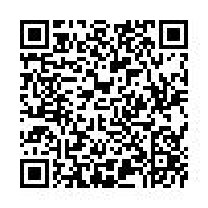
\includegraphics[height=0.3\textwidth]{img/QR/perfect_03.jpg}
  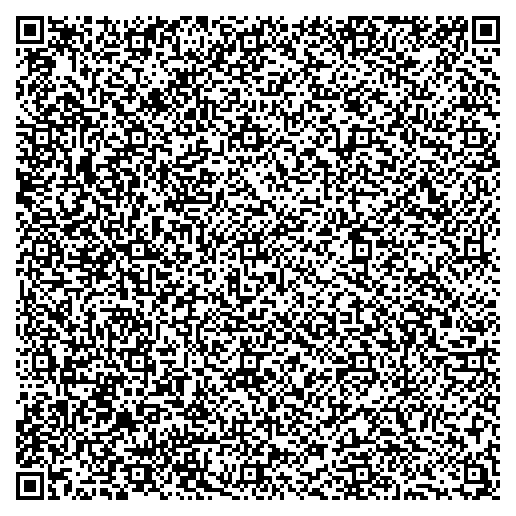
\includegraphics[height=0.3\textwidth]{img/QR/perfect_02.png}
  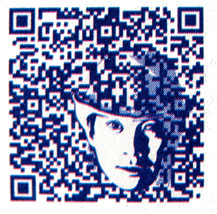
\includegraphics[height=0.3\textwidth]{img/QR/perfect_04.jpg}
  \caption{normale Größe, groß, mit enthaltenem Bild}
  \label{fig:qrnormal}
\end{figure}

% unscharfe
Auch Bilder, die mit einem Gaußschen Weichzeichner unscharf gemacht wurden, werden bis zu einem Radius von 3 Pixeln noch gut erkannt. Ab etwa 3,5 Pixeln sind die Kanten allerdings, wie in Abbildung \ref{fig:qrblur} zu sehen ist, zu unscharf und der Code kann nicht dekodiert werden.
\begin{figure}[H]
  \centering
  
\includegraphics[width=0.3\textwidth]{img/QR/blurry_03_3.jpg}
  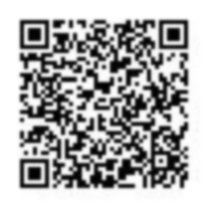
\includegraphics[width=0.3\textwidth]{img/QR/blurry_03_35f.jpg}
  \caption{\surname{Gauß}'scher Weichzeichner mit 3,0 Pixeln und 3,5 Pixeln Radius}
  \label{fig:qrblur}
\end{figure}

% rotierte und rotiert+unscharf
In Abbildung \ref{fig:qrrotate} sind rotierte QR-Codes abgebildet, dabei sieht man im ersten Bild eine 45$ ^\circ $ Drehung, da die Rotation des Bildes bei vollständigen QR-Codes unwichtig ist, das Bild wird immer akzeptiert. Allerdings können Fehler oder Überdeckungen dazu führen, dass Rotationen nur eingeschränkt durchführbar sind, wie z.B. beim Bild im Code~(Bild 2/3), wo nur bis 25$^\circ$ und dann wieder ab 63$^\circ$ der Code erkannt wird.

Natürlich betrifft das auch unscharfe Bilder, die ebenfalls nicht bei jedem Drehwinkel erkannt werden. Das sieht man z.B. in Bild 4, wo mit 35$^\circ$ der Code noch erkannt wird, und in Bild 5, wo der um 40$^\circ$ gedrehte Code nicht mehr erkannt wird.
\begin{figure}[H]
  \centering
  \setlength{\fboxrule}{1pt}
  \fbox{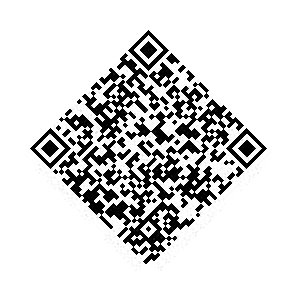
\includegraphics[height=0.3\textwidth]{img/QR/rotated_03_45.jpg}}
  \fbox{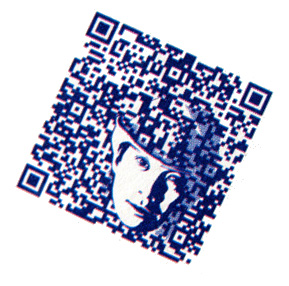
\includegraphics[height=0.3\textwidth]{img/QR/rotated_04_25.jpg}}
  \fbox{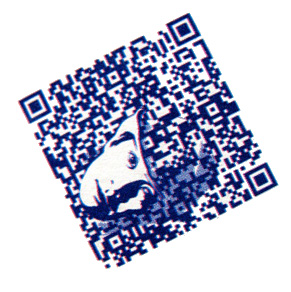
\includegraphics[height=0.3\textwidth]{img/QR/rotated_04_63.jpg}}
  \fbox{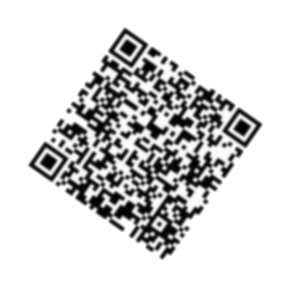
\includegraphics[height=0.3\textwidth]{img/QR/blurryrotate_03_3_35.jpg}}
  \fbox{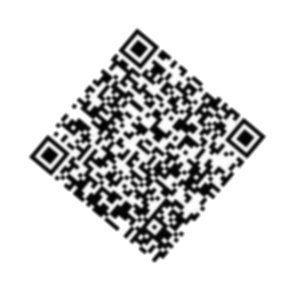
\includegraphics[height=0.3\textwidth]{img/QR/blurryrotate_03_3_40f.jpg}}
  \caption{Rotationen mit 45$^\circ$, 25$^\circ$, 63$^\circ$, 35$^\circ$ und 40$^\circ$}
  \label{fig:qrrotate}
\end{figure}

% dunkle, dunkle+Fehler, dunkle+unscharf, dunkle+rotiert und dunkle+unscharf+rotiert
Die allgemeine Dunkelheit des Bildes, durch die der Kontrast sinkt, scheint kaum Auswirkungen auf die Erkennung der QR-Codes zu haben. Bei vollständigen Codes kann bis zu einer Abdunklung von 98\% immer noch der Code übersetzt werden, wobei selbst das menschliche Auge schon kaum noch etwas erkennen kann~(siehe Abbildung \ref{fig:qrdark}, Bild 1). Auch bei Codes mit integrierten Bildern ist, wie bei um 45$ ^\circ $ gedrehten Codes, eine Abdunklung bis zu 90\% kein Problem. Sogar bei maximal unscharfen und zusätzlich maximal gedrehten Codes ist eine Abdunklung von bis zu 90\% möglich.
\begin{figure}[H]
  \centering
  
\includegraphics[height=0.3\textwidth]{img/QR/dark_03_98.jpg}
  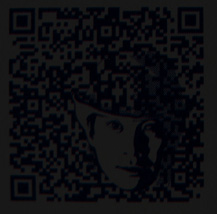
\includegraphics[height=0.3\textwidth]{img/QR/dark_04_90.jpg}
  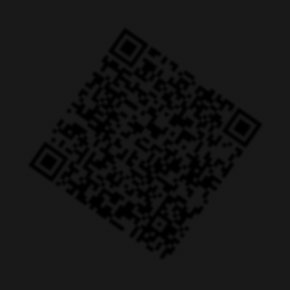
\includegraphics[height=0.3\textwidth]{img/QR/blurrydarkrotate_03_3_90_35.jpg}
  \caption{abgedunkelte Bilder: Bei 98\%, mit Bild bei 90\%, rotiert+unscharf bei 90\%}
  \label{fig:qrdark}
\end{figure}

% schatten
Leicht schattige Bilder, bis 60\% Abdunklung im Schatten, können bei jeglicher Überdeckungsrate gut erkannt werden. Ab 80\% Abdunklung sind allerdings kaum noch Codes dekodierbar, es sei denn, der Schattenbereich ist durch die Fehlerkorrektur des Codes ausgleichbar. Sich überlagernde Schatten, sind als jeweils einzelne Schatten anzusehen und können auch als solche bearbeitet werden.
\begin{figure}[H]
  \centering
  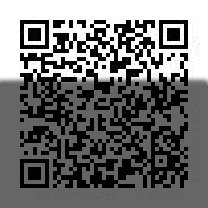
\includegraphics[height=4cm]{img/QR/shade_03_60+60.jpg}
  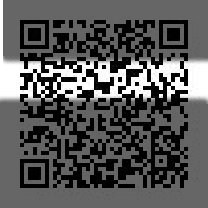
\includegraphics[height=4cm]{img/QR/shade_03_2x60.jpg}
  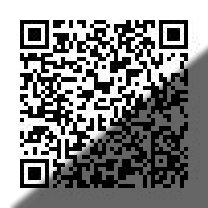
\includegraphics[height=4cm]{img/QR/shade_03_60+s40.jpg}
  \caption{Schatten, die jeweils um 60\% abdunkeln}
  \label{fig:qrshade}
\end{figure}
